%% Apuntes de Fotodeteccion y Trayectorias Cuanticas
%
%\documentclass[twocolumn]{article}
\documentclass[twocolumn,aps,eqsecnum,showkeys,amsmath]{revtex4}
\usepackage[spanish,activeacute]{babel}
\usepackage{graphicx}
\usepackage{amsmath}
\usepackage{color}
\usepackage{cancel}

% vectors (the most common ones)
\newcommand{\mbi}{\mathbf{i}}
\newcommand{\mbj}{\mathbf{j}}
\newcommand{\mbk}{\mathbf{k}}
\newcommand{\mbp}{\mathbf{p}} 
\newcommand{\mbq}{\mathbf{q}}
\newcommand{\mbr}{\mathbf{r}}
%\newcommand{\mbrp}{\mathbf{r}^{\prime}}
\newcommand{\mbv}{\mathbf{v}}
\newcommand{\mbE}{\mathbf{E}}
\newcommand{\mbR}{\mathbf{R}}

\newcommand{\mcC}{\mathcal{C}} 
\newcommand{\mcH}{\mathcal{H}} 	%Hamiltonian
\newcommand{\mcL}{\mathcal{L}} 	
\newcommand{\mcS}{\mathcal{S}} 
\newcommand{\mcE}{\mathcal{E}} 
\newcommand{\mcV}{\mathcal{V}} 	%Hamiltonian
\newcommand{\Tr}{\mathrm{Tr}}
\newcommand{\qed}{\mathrm{Q.E.D.}}
\newcommand{\p}{\partial}
%\newcommand{\lan}{\langle}     \newcommand{\ran}{\rangle}
\newcommand{\adg}{a^{\dag}}
\newcommand{\Adg}{A^{\dag}} 	
\newcommand{\Hdg}{H^{\dag}} 	 
\newcommand{\Udg}{U^{\dag}} 	

\newcommand{\lan}{\langle}
\newcommand{\ran}{\rangle}
%\newcommand{\adg}{a^{\dag}}

\providecommand{\abs}[1]{\left\lvert#1\right\rvert}
\providecommand{\norm}[1]{\lVert #1 \rVert}
\providecommand{\vxp}[1]{\langle #1 \rangle}
\providecommand{\bra}[1]{\langle #1 \rvert}
\providecommand{\ket}[1]{\lvert #1 \rangle}
\providecommand{\bbra}[1]{\langle #1 \rvert\rvert}
\providecommand{\kket}[1]{\lvert\lvert #1 \rangle}
\providecommand{\kkket}[1]{\lvert #1 \rangle\rangle}
\providecommand{\braket}[2]{\langle #1 \rvert #2 \rangle}
%\providecommand{\vxp3}[3]{\langle #1 |#2| #3 \rangle}
\providecommand{\tr}[1]{\text{tr}\left[ #1 \right]}
\newcommand{\ketbra}[2]{\left| {#1} \right\rangle\left\langle {#2}\right|}
%\newcommand{\mmax}{_{\text{max}}}

\newcommand{\mru}[1]{\mathrm{#1}} %unidades fisicas
\newcommand{\inc}[1]{\mathrm{(#1)}} %incisos en formulas desplegadas
\newcommand{\tbn}[1]{\textbf{#1}} %numero de problema

\begin{document}

\title{Trayectorias Cu\'anticas para Fluorescencia Resonante Intermitente: 
$^{171} \mathrm{Yb}^+$}
\author{H\'ector M. Castro Beltr\'an}
\affiliation{Centro de Investigaci\'on en Ingenier\'ia y 
Ciencias Aplicadas, IICBA, \\ Universidad Aut\'onoma del Estado de Morelos,  
Av. Universidad 1001, 62209 Cuernavaca, Morelos, M\'exico}

\date{\today}
\begin{abstract} 
Apuntes en proceso. En estos apuntes hacemos una tratamiento de teor\'ia 
de trayectorias cu\'anticas para la fluorescencia resonante intermitente (FRI) 
de un \'atomo de tres niveles excitado por un l\'aser. El l\'aser excita una 
transici\'on dipolar fuerte en la que se emiten muchos fotones (per\'iodo 
brillante); el estado excitado decae tambi\'en a un estado metaestable, 
provocando per\'iodos sin fluorescencia de la transici\'on fuerte (per\'iodo 
oscuro).  Simulamos mediciones de luz mediante ecuaciones estoc\'asticas 
de Schr\"odinger, que son ecuaciones para la evoluci\'on de la funci\'on de 
onda. Estos m\'etodos son llamados Trayectorias Cu\'anticas o de Funci\'on 
de Onda de Monte Carlo, y engloban m\'etodos de saltos cu\'anticos y 
difusi\'on de estados cu\'anticos para tratar fotoconteo, detecci\'on homodina 
y heterodina y  detecci\'on de espectros. 
\end{abstract}

\keywords{Quantum trajectories, quantum jumps, quantum state diffusion, 
homodyne and heterodyne measurements, intensity correlations, 
amplitude-intensity correlation, resonance fluorescence}
\maketitle

%%%%%%%%10%%%%%%%%20%%%%%%%%30%%%%%%%%40%%%%%%%%50%%%%%%%%60%%%%%%%%70%%%
\section{Introducci\'on}
\subsection{Comments}
These notes are meant as a compilation of the main QT approaches to RF 
for use in class. The notes are limited to the very basics (of the physics and 
theory of QTs) but hopefully the students will be able to develop their own 
computer codes. 

Intensity, intensity-intensity correlations, waiting-time distribution, 
photoelectron statistics and sub-Poissonian statistics, are measured by 
direct photon counting, simulated by discontinuous trajectories (Quantum 
jumps, QJ). 
Homodyne and heterodyne detection, simulated by quantum state diffusion 
(QSD) trajectories, allow phase-dependent measurements of the field, such 
as single-quadrature, and squeezing, among other things. CHD mixes QJs 
and QSD to provide a new look at quantum fluctuations and resolves 
squeezing in a detector-efficiency-independent manner. Spectra can be 
measured by homodyne, heterodyne and filtered measurements 
\cite{TiCa92,Holl97}. 

Quantum trajectories, as formulated by Carmichael, simulate the output of 
an experiment, and a large ensemble of trajectories represents the average 
result of many experiments. 

More on quantum open systems \ldots Our system consists of a coherent 
part that features the atom-laser coupling. This is often studied with an 
unitary evolution via the Schr\"odinger equation. However, the coupling of 
the atom to the environment leads to dissipation, thus forcing a density 
operator approach (master equation) or a Heisenberg-Langevin approach. 

\subsection{Evolution of a Quantum Open System} %%%%%%%%%%%%%%%
In resonance fluorescence we have an atomic system driven by lasers and 
maybe also by cavity fields. Magnetic fields are often added to prepare the 
atomic system in a specific state. To simplify matters we mostly speak of the 
interaction of a single two-level atom of transition frequency $\omega_a$ 
with a single monochromatic laser treated classically (not an operator). The 
atom-laser coupling is given by the Rabi frequency $\Omega$  The (RWA) 
Hamiltonian in the frame rotating at the laser frequency is 
%
\begin{equation}
H_0 = \Delta \sigma_{ee} +\frac{\Omega}{2}(\sigma_+  +\sigma_-)  \,,
\end{equation}
%%
where $\sigma_i$ are Pauli spin operators, and$\Delta= \omega_a -\omega$ 
is the atom-field detuning ($\hbar=1$). The state of the atom is given by the 
wave function $\ket{\Psi (t)} = c_g(t) \ket{g} +c_e(t) \ket{e}$. 

The atom is also coupled to a large reservoir of harmonic oscillators which 
induce  decay of the excited state at the rate $\gamma$. At optical 
frequencies and room temperatures (and below)  we can neglect blackbody 
radiation effects. The full atom-laser-reservoir is described by the master 
equation 
%
\begin{eqnarray} 	\label{MasterEq}
\dot{\rho} &=& - i [H_0,\rho] +\frac{\gamma}{2} \left[ 2 \sigma_- \rho \sigma_+ 
	-\sigma_+ \sigma_- \rho - \rho  \sigma_+ \sigma_- \right]  	\,. 		
\end{eqnarray}
%%

The master equation can be unraveled in an infinite number of ways but only 
a limited number of them have an experimental significance, each looking at 
different properties. The decomposition above is suitable for direct 
photodetection simulation, it corresponds to a discontinuous evolution of the 
wave function due to photon emissions (quantum jumps); this deals with the 
particle aspect of light  \cite{Carm93,DaCM92,DuZR92}. We later deal with 
homodyne and heterodyne measurements (wave features -- quantum 
diffusion) \cite{Carm93,Carm96,WiMi93a,WiMi93b,Perc98}. Also spectral 
detection \cite{TiCa92,Holl97}. 

%%%%%%%%%%%%%%%%%%%%%
\subsection{Distribuci\'on de Tiempos de Espera de Fluorescencia 
Resonante de un \'Atomo de Dos Niveles} 
\tbn{Carmichael SMQO1 2.6} La distribuci\'on de tiempos de espera de fotoelectrones de fluorescencia resonante para eficiencia de detecci\'on 
unidad esta dada por 
$$ w_{ss}(\tau) = \frac{\gamma Y^2}{2Y^2-1} e^{-\gamma \tau/2}
	(1- \cos{\delta' \tau}) \,,$$
donde $\delta' \equiv (\gamma/2) \sqrt{1-2Y^2}$ y 
$Y=\sqrt{2} \Omega/\gamma$. 
(b) Se satisface que $\int_0^{\infty} w_{ss}(\tau) d\tau =1$. 
(c) El intervalo medio entre fotopulsos es $\overline{\tau} 
=2(1+Y^2)/\gamma Y^2 =(\gamma \langle \sigma_+ \sigma_- \rangle )^{-1}$. 

%%%%%%%%10%%%%%%%%20%%%%%%%%30%%%%%%%%40%%%%%%%%50%%%%%%%%60%%%%%%%%70%%%
\section{El i\'on $^{171} \mathrm{Yb}^+$}
%
\begin{figure}[b]
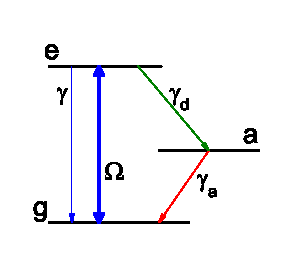
\includegraphics{3LA_onelaser.pdf} 
\caption{ \label{fig:3LA} 
Scheme of the three-level atom-laser interaction and spontaneous 
decay rates. }
\end{figure}
%% 

Hamiltoniano \'atomo-l\'aser 
%
\begin{equation}
H_0 = \Delta \sigma_{ee} +\frac{\Omega}{2}(\sigma_{eg}  +\sigma_{ge})  \,,
\end{equation}
%%
donde $\sigma_{jk}$ son operadores del \'atomo, y  
$\Delta= \omega_{eg} -\omega$ es la desinton\'ia del l\'aser con la frecuencia 
de la transici\'on ($\hbar=1$). El estado del \'atomo est\'a dado por la funci\'on 
de onda no normalizada 
%
\begin{equation}
\ket{\bar{\Psi} (t)} = \bar{c}_g(t) \ket{g} +\bar{c}_e(t) \ket{e} 
	+\bar{c}_a(t) \ket{a} \,,
\end{equation}
%%

Requerimos resolver la ecuaci\'on de Schr\"odinger no unitaria
%
\begin{equation}
\ket{\dot{\Psi}} = -i \mathcal{H} \ket{\Psi} \,,
\end{equation}
%%
donde 
%
\begin{eqnarray}
H_{\mathrm{eff}} = \mathcal{H} =
H_0 -i \frac{\gamma}{2} \sigma_{ee} 
	-i \frac{\gamma_d}{2} \sigma_{ee} -i \frac{\gamma_a}{2} \sigma_{aa} \,, 
\end{eqnarray}
%%
es un Hamiltoniano efectivo. Entonces, las ecuaciones para las amplitudes 
son:   
%
\begin{subequations}
\label{eq:jumpSSEamp}
\begin{eqnarray}
\dot{\bar{c}}_e &=& -i \frac{\Omega}{2} \bar{c}_g  
	-\left( \frac{\gamma +\gamma_d}{2} +i \Delta \right) \bar{c}_e \\ 
%
\dot{\bar{c}}_g &=& -i \frac{\Omega}{2} \bar{c}_e  \\
%
\dot{\bar{c}}_a &=& -i\frac{\gamma \bar{c}_a}{2} \,.    
\end{eqnarray}
\end{subequations}
%%
%
%\begin{subequations}
%\label{eq:jumpSSEampSol}
%\begin{eqnarray}
%\dot{c}_e &=&  \\ 
%
%\dot{c}_g &=&   \\
%
%\dot{c}_a &=& e^{-\gamma_a t/2} c_a(0) \,.    
%\end{eqnarray}
%\end{subequations}
%%
Las soluciones solamente expresan la evoluci\'on de la funci\'on de onda 
entre dos emisiones consecutivas de fotones. 

La emisi\'on de un fot\'on interrumpe la evoluci\'on, colapsando la funci\'on 
de onda. Por ejemplo, sea $\mathcal{C} = \sqrt{\gamma} \sigma_{ge}$ el 
operador que indica la emisi\'on de un fot\'on en la transici\'on 
$\ket{e} - \ket{g}$, entonces  
%
\begin{equation}
\ket{\bar{\Psi}_c} \to \mathcal{C} \ket{\bar{\Psi}_c} 
	= \sqrt{\gamma} c_e \ket{g} \,. 
\end{equation}
%%

Para incluir los procesos 
aleatorios de emisi\'on espont\'anea debemos calcular primero las 
probabilidades de emisi\'on de un fot\'on para cada una de las transiciones: 
%
\begin{eqnarray}
p_k(t) &=& \delta t \bra{\Psi_c (t)} \mcC_k^\dag \mcC_k \ket{\Psi_c (t)} 	\,,
\end{eqnarray}
%%
donde 
%
\begin{equation}
\mcC_e = \sqrt{\gamma} \sigma_{ge} \,, \quad 
	\mcC_d = \sqrt{\gamma_d} \sigma_{ae} \,, \quad 
	\mcC_a = \sqrt{\gamma_a} \sigma_{ga} \,, 
\end{equation}
%%
son operadores de colapso y $\ket{\Psi_c (t)}$ es la funci\'on de onda 
(normalizada) con una historia particular de colapsos mediados por 
per\'iodos de evoluci\'on cont\'inua.  Estas probabilidades deben ser 
comparadas con n\'umeros aleatorios $r_k \in (0,1)$. Si $p_k(t) > r_k$ 
se produce la emisi\'on de un fot\'on; de lo contrario, la funci\'on de onda 
evoluciona de forma cont\'inua. Cada intervalo de tiempo se realiza esta 
comparaci\'on.  

La normalization de la funci\'on de onda se realiza mediante 
%
\begin{eqnarray}
\ket{\Psi_c} &=& \frac{ \ket{\bar{\Psi}_c} }
	{ \sqrt{ \braket{ \bar{\Psi}_c}{\bar{\Psi}_c}  }  } \,, \\ 
\braket{ \bar{\Psi}_c}{\bar{\Psi}_c} &=& |\bar{c}_e|^2 +|\bar{c}_a|^2 
	+|\bar{c}_g|^2	\,.
\end{eqnarray}
%%


El procedimiento muestra lo que llamamos una Trayectoria Cu\'antica 
o evoluci\'on de la funci\'on de onda estoc\'astica. En la Fig.1 mostramos 
un ejemplo de trayectoria, en la que se aprecian los per\'iodos brillantes, 
per\'iodos de emisi\'on frecuente de fotones, y per\'iodos oscuros, donde 
no hay emisi\'on de fotones. Por la naturaleza aleatoria del proceso, en el 
c\'alculo de un promedio, diferentes trayectorias se superponen y borran la 
 discontinuidad de una trayectoria. Un n\'umero muy grande de trayectorias 
 reproducen el resultado obtenido con el operador de densidad. 
 
 Para el siguiente reporte de la estancia deseamos obtener las 
 distribuciones de las duraciones de los per\'iodos brillantes y oscuros y 
 sus respectivos valores promedio. 


%
\begin{eqnarray}
p_k(t) &=& \delta t \bra{\Psi_c (t)} \mcC_k^\dag \mcC_k \ket{\Psi_c (t)} 	\\
p_e(t) &=& \gamma\, \delta t \, 
	\frac{|c_e(t)|^2}{|c_g(t)|^2 +|c_e(t)|^2 +|c_a(t)|^2} \,, \\
p_d(t) &=& \gamma_d\, \delta t \, 
	\frac{|c_e(t)|^2}{|c_g(t)|^2 +|c_e(t)|^2 +|c_a(t)|^2} \,, \\
p_a(t) &=& \gamma_a\, \delta t \, 
	\frac{|c_a(t)|^2}{|c_g(t)|^2 +|c_e(t)|^2 +|c_a(t)|^2} \,,
	\end{eqnarray}
%%


%%%%%%%%10%%%%%%%%20%%%%%%%%30%%%%%%%%
\subsection{Algoritmo para determinar las distribuciones de per\'iodos 
brillantes y oscuros}
Se requiere una trayectoria muy larga ($\gamma T \sim 10^5 - 10^6$) 
que contenga $\sim 10^2$ per\'iodos brillantes (PB) y oscuros (PO).
\textcolor{red}{
Posteriormente, calcular distribuciones de n\'umero de fotones 
(trayectorias m\'as cortas) y de tiempos de retardo.}  
%
\begin{itemize}
\item La condici\'on inicial es \'atomo en su estado base, 
$\bar{c}_g (0) =1, \, \bar{c}_e (0) = \bar{c}_a (0) =0$. Contador de 
PB y PO: $n_B = n_O =0$. Contador de saltos $n_S=0$
%
\item Inicia reloj de la trayectoria, $t_i=idt$, $i=0,1,2,\ldots,i_{max}$, 
$t_{imax} = T = i_{max} dt$. 
%
\item Inicia reloj de duraci\'on de un PB, $t_j = jdt$, $j=0,1,2,\ldots$ 
(no hay $j_{max}$ fijo). (Comentario: es muy probable que se desarrolle 
un PB bien definido al principio.) 
%
\item Propagar de acuerdo al algoritmo de trayectorias discont\'inuas.   
Incrementar n\'umero de brincos $n_S = n_S +1$. 
%
\item Calcular duraci\'on $t_B$ del PB. Guardar $t_B$ cuando 
$p_d > r_d$ (fin del PB). Agregar n\'umero de PB, $n_B = n_B+1$. 
%
\item Si $p_d > r_d$ se entra a a un PO, durante el cual 
$\bar{c}_a (0) =1, \, \bar{c}_e (0) = \bar{c}_g (0) =0$. 
%
\item Inicia reloj de duraci\'on de un PO, $t_k = kdt$, $k=0,1,2,\ldots$ 
(no hay $k_{max}$ fijo).
%
\item Propagar de acuerdo al algoritmo de trayectorias discont\'inuas   
%
\item Calcular duraci\'on $t_O$ del PO. Guardar $t_O$ cuando 
$p_a > r_a$ (fin del PO). Termina PO. 
%
\item Repetir procedimiento hasta que $t_i = t_{imax} =T$. 
Descartar \'ultimo per\'iodo (brillante u oscuro), que queda truncado, 
para no alterar la distribuci\'on. 
%
\item Construir las distribuciones de PB y PO. Obtener TB y TO. 
Comparar con la forma exponencial esperada $P_B \sim e^{-t/TB}$, 
$P_O \sim e^{-t/TO}$. \textcolor{red}{Sugerencia: Para los histogramas 
agrupar $t_B, t_O$ en \textit{bins} de duraciones de varios $dt$. Por 
ejemplo, bins de $5dt$: $j_1=k_1=1,2,3,4,5$, $j_2=k_2=6,7,8,9,10$, etc.}
\end{itemize}
%%

\textcolor{blue}{Localizar art\'iculo donde se obtiene que las distribuciones 
de PO y PB tienen forma exponencial.}


%%%%%%%%10%%%%%%%%20%%%%%%%%30%%%%%%%%40%%%%%%%%50%%%%%%%%60%%%%%%%%70%%%
\section{Trayectorias Cu\'anticas: Introducci\'on}
These notes are meant as a compilation of the main QT approaches to 
RF for use in class. The notes are limited to the very basics (of the physics 
and theory of QTs) but hopefully the students will be able to develop their 
own computer codes. 

Intensity, intensity-intensity correlations, waiting-time distribution, 
photoelectron statistics and sub-Poissonian statistics, are measured by 
direct photon counting, simulated by discontinuous trajectories (QJ). 
Homodyne and heterodyne detection, simulated by quantum state 
diffusion  trajectories, allow phase-dependent measurements of the field, 
such as single-quadrature, and squeezing, among other things. CHD 
mixes QJs and QSD to provide a new look at quantum fluctuations and 
resolves squeezing in a detector-efficiency-independent manner. Spectra 
can be measured by homodyne, heterodyne and filtered measurements 
\cite{TiCa92,Holl97}. 

Quantum trajectories, as formulated by Carmichael, simulate the output 
of an experiment, and a large ensemble of trajectories represents the 
average result of many experiments. 

More on quantum open systems \ldots Our system consists of a coherent 
part that features the atom-laser coupling. This is often studied with an 
unitary evolution via the Schr\"odinger equation. However, the coupling of 
the atom to the environment leads to dissipation, thus forcing a density 
operator approach (master equation) or a Heisenberg-Langevin approach. 

\subsection{Evolution of a Quantum Open System} %%%%%%%%%%%
In resonance fluorescence we have an atomic system driven by lasers 
and maybe also by cavity fields. Magnetic fields are often added to prepare 
the atomic system in a specific state. To simplify matters we mostly speak 
of the interaction of a single two-level atom of transition frequency 
$\omega_a$ with a single monochromatic laser treated classically (not an 
operator). The atom-laser coupling is given by the Rabi frequency 
$\Omega$  The (RWA) Hamiltonian in the frame rotating at the laser 
frequency is 
%
\begin{equation}
H_0 = \Delta \sigma_{ee} +\frac{\Omega}{2}(\sigma_+  +\sigma_-)  \,,
\end{equation}
%%
where $\sigma_i$ are Pauli spin operators, and 
$\Delta= \omega_a -\omega$ is the atom-field detuning ($\hbar=1$). 
The state of the atom is given by the wave function 
$\ket{\Psi (t)} = c_g(t) \ket{g} +c_e(t) \ket{e}$. 

The atom is also coupled to a large reservoir of harmonic oscillators 
which induce decay of the excited state at the rate $\gamma$. At optical 
frequencies and room temperatures (and below)  we can neglect 
blackbody radiation effects. The full atom-laser-reservoir is described by 
the master equation 
%
\begin{eqnarray} 	\label{MasterEq}
\dot{\rho} &=& - i [H_0,\rho] +\frac{\gamma}{2} \left[ 2 \sigma_- \rho \sigma_+ 
	-\sigma_+ \sigma_- \rho - \rho  \sigma_+ \sigma_- \right]  	\,. 		
\end{eqnarray}
%%

The master equation can be unraveled in an infinite number of ways but 
only a limited number of them have an experimental significance, each 
looking at different properties. The decomposition above is suitable for 
direct photodetection simulation, it corresponds to a discontinuous 
evolution of the wave function due to photon emissions (quantum jumps); 
this deals with the particle aspect of light  \cite{Carm93,DaCM92,DuZR92}. 
We later deal with homodyne and heterodyne measurements (wave 
features -- quantum diffusion) 
\cite{Carm93,Carm96,WiMi93a,WiMi93b,Perc98}. Also spectral detection \cite{TiCa92,Holl97}. 


%%%%%%%%10%%%%%%%%20%%%%%%%%30%%%%%%%%40%%%%%%%%50%%%%%%%%60%%%%%%%%70%%%
\section{Trayectorias Discont\'inuas: Detecci\'on por Fotoconteo 
(M\'etodo de Brincos Cu\'anticos)}
En este caso la luz se recolecta por detecci\'on directa de los fotones por 
fotodetectores de banda ancha. Escribimos la ecuaci\'on maestra como 
%
\begin{eqnarray} 	\label{MasterEqEffJ}
\dot{\rho} &=& \mcL \rho = - i ( \mcH \rho -\rho \mcH^{\dag} )  +\mcS \rho \,, 
\end{eqnarray}
%%
donde a $\mcL$ se llama superoperador de Lindblad, 
%
\begin{eqnarray} 
\mcH &=& H_0 - i \frac{\gamma}{2} \sigma_+ \sigma_-   
\end{eqnarray}
%%
es un Hamiltoniano efectivo no Hermitiano, y  
%
\begin{eqnarray} 
\mcS \rho &=& \gamma \sigma_- \rho \sigma_+ 
\end{eqnarray}
%%
es llamado \textit{el operador de brinco}, que corresponde a un evento de 
emisi\'on espont\'anea. Esto es porque  
$\gamma \sigma _+ \rho \sigma_ - = \gamma \rho_{ee} \sigma_{gg}$, es decir,  
el operador de brinco disminuye el estado del \'atomo. 

La soluci\'on formal  de la ecuaci\'on maestra es $\rho(t) = e^{\mcL t} \rho (0)$. 
Con la descomposici\'on (\ref{MasterEqEffJ}) podemos escribir 
%
\begin{eqnarray} 	%\label{MasterEqEffJ}
\dot{\rho} &=& ( \mcL - \mcS ) \rho  +\mcS \rho \,. 		
\end{eqnarray}
%%
La soluci\'on 
%
\begin{eqnarray} 	%\label{MasterEqEffJ}
\rho (t) &=& e^{ [( \mcL - \mcS ) +\mcS ] t} \rho (0)  	\nonumber \\ 
&=& 	\sum_{m=0}^{\infty} \int_0^t dt_m  \int_0^{t_m} dt_{m-1}  \cdots 	
	 \int_0^{t_2} dt_1 e^{ (\mcL - \mcS) (t-t_m)}  		\nonumber \\ 
	&& \mcS e^{ (\mcL - \mcS) (t_m-t_{m-1})} \mcS \cdots 
	\mcS  e^{ (\mcL - \mcS) t_1} \rho(0) \,,
\end{eqnarray}
%%
no es dif\'icil de entender \cite{Carm93}. El integrando es el operator de densidad condicional no normalizado  $\bar{\rho}_c (t)$ 
%
\begin{eqnarray} 	\label{eq:condDensOp}
\bar{\rho}_c (t) &=& e^{ (\mcL - \mcS) (t-t_m)} \mcS 	
	 e^{ (\mcL - \mcS) (t_m-t_{m-1}} \mcS 	\nonumber \\  
	&&\cdots \mcS  e^{ (\mcL - \mcS) t_1} \rho(0) \,,
\end{eqnarray}
%%
para el estado inicial $\rho_c (0) = \rho (0)$. Esta serie es una suma sobre diferentes 
historias de fotoemisiones de la fuente desde $t=0$ hasta $t$. Cada historia es 
\'unica y puede involucrar cualquier n\'umero de fotoemisiones, desde $m=0$ hasta $m=\infty$, y los tiempos de las emisiones pueden ser cualquier secuencia ordenada 
de $m$ veces en el intervalo $[0,t]$.  La interpretaci\'on f\'isica de $\bar{\rho}_c (t)$ 
es de evoluciones sin fotoemisiones interrumpidas por \textit{colapsos} del estado a 
los tiempos de emisi\'on. Al tiempo $t$, para un estado inicial $\rho (0)$ y una 
secuencia particular de tiempos de emisi\'on, el operador de densidad condicionado 
de la fuente esta dado por 
%
\begin{eqnarray} 	\label{eq:condDensOp}
\rho_c (t) &=& \frac{\bar{\rho}_c (t) }{ \Tr [\bar{\rho}_c (t) ]} \,.
\end{eqnarray}
%%

Cada secuencia o historia de fotoemisiones se llama \textit{trayectoria cu\'antica}. 
Este tipo de trayectorias de fotoemisiones (detecci\'on directa)  se denomina en 
ingl\'es \textit{unraveling}, una descomposici\'on particular del operador de densidad. 
Existen otras descomposiciones que corresponden a otros m\'etodos de medici\'on 
de la luz. 

N\'otese que mientras que $\rho (t)$ llega a un  estado estacionario, $\rho_c (t)$ 
no lo har\'a; cada trayectoria mantiene su evoluci\'on estoc\'astica. La trayectoria, 
sin embargo, es estacionaria en sentido estad\'istico, y el estado estacionario 
para $\rho$ puede calcularse como un promedio en el tiempo de $\rho_c (t)$. 

Para muchos sistemas el Hamiltoniano permite factorizar el operador 
de densidad en estados puros
%
\begin{eqnarray}
\rho_c (t) &=& \ketbra{\Psi_c (t) }{ \Psi_c  (t)} 	\,, 	\quad 
	\bar{\rho}_c (t) = \ketbra{ \bar{\Psi}_c (t) }{ \bar{\Psi}_c  (t)} \,, 
	\nonumber \\ 
\end{eqnarray}
%%
Mas adelante veremos algunos ejemplos. Entonces reemplazamos el propagador 
$e^{ (\mcL - \mcS) \Delta t}$ del operador de densidad $\bar{\rho}_c (t)$ por el de 
la funci\'on de onda $| \bar{\Psi}_c (t) \rangle$. La propagaci\'on sin fotoemisi\'on 
en un tiempo $\Delta t$ esta dada por 
%
\begin{eqnarray}
\ket{ \bar{\Psi}_c (t+ \Delta t) } 
	= e^{- i \mcH \Delta t /\hbar} \ket{ \bar{\Psi}_c (t) } 
\end{eqnarray}
%%
que es la soluci\'on de la ecuaci\'on de Schr\"odinger 
%
\begin{eqnarray}
i \frac{d}{dt} \ket{ \bar{\Psi}_c } = {\cal H} \ket{ \bar{\Psi}_c } \,,
\end{eqnarray}
%%
donde $\ket{ \bar{\Psi}_c }$ es una funci\'on de onda no-normalizada debida a la 
acci\'on del Hamiltoniano no Hermitiano $\mcH$ que lleva a una evoluci\'on 
no unitaria, asegurando la p\'erdida de probabilidad de que el \'atomo se encuentre 
en el estado excitado. 

Escribamos la funci\'on de onda como 
%
\begin{equation}
\ket{ \bar{\Psi}_c (t) } = c_g(t) \ket{g} +c_e(t) \ket{e} 	\,,
\end{equation}
%%
La funci\'on de onda normalizada es 
$$\ket{ \Psi_c(t) } = \ket{ \bar{\Psi}_c(t) } / 
	[\braket{ \bar{\Psi}_c(t)}{ \bar{\Psi}_c(t)} ]^{1/2} \,.$$
El sistema \'atomo-campo evoluciona de manera cont\'inua pero no unitaria por un 
per\'iodo de tiempo hasta que se emite un fot\'on espont\'aneamente, se\~nalando 
el regreso del \'atomo al estado base. Este ciclo se repite durante una historia. 

Al tiempo $t_j$ en el que ocurre una emisi\'on el estado no normalizado 
experimenta un colapso dado por el operador de brinco 
$\mcC = \sqrt{\gamma}\, \sigma_-$,  
%
\begin{equation}
\ket{ \bar{\Psi}_c } \to \mcC \ket{ \bar{\Psi}_c } 
	= \sqrt{\gamma}\, c_e (t_j) \ket{g} 	\,,
\end{equation}
%%
que se normaliza como 
 %
\begin{eqnarray} 	\label{jump}
\ket{\Psi_c(t_j)} = \frac{\mcC \ket{\Psi_c(t_j) } }
  	 {\sqrt{\bra{\Psi_c(t_j)}  \mcC^\dag \mcC \ket{\Psi_c(t_j)} } } \,,	
\end{eqnarray}
%%
y que ocurre con probabilidad en el intervalo $[t, t+ \delta t]$ 
%
\begin{eqnarray} 	\label{JumpProb}
p_c(t) &=& \delta t \bra{\Psi_c (t)} \mcC^\dag \mcC \ket{\Psi_c (t)} 	\\ 
	&=& \gamma \delta t \bra{\Psi_c (t)} \sigma_+ \sigma_- \ket{\Psi_c (t)}
	\nonumber \,.
\end{eqnarray}
%%

Entonces, una simulaci\'on num\'erica ocurre en el tiempo discreto con paso 
$\delta t$. Obtenemos una trayectoria estoc\'astica para la funci\'on de onda 
$\ket{\Psi_c (t_n)}$, donde $t_n = n \delta t$. Dada $\ket{\Psi_c (t_n)}$, la 
funci\'on de onda $\ket{\Psi_c (t_{n+1})}$ se obtiene con el siguiente algoritmo: 
\newline (i) Evaluar la probabilidad de un brinco $p_c (t_n)$. 
\newline (ii) Generar un n\'umero aleatorio $r_n$ distribuido uniformemente en el intervalo $[0,1]$. 
\newline (iii) Comparar $p_c(t_n)$ con $r_n$ y calcular  $\ket{\Psi_c (t_{n+1})}$ 
de acuerdo a la regla   
 %
\begin{subequations}
\begin{eqnarray*} 	%\label{jump}
\ket{\Psi_c(t_{n+1}) } &=& \frac{\mcC \ket{\Psi_c(t_n) } } 
	{\sqrt{\bra{\Psi_c(t_n)} \mcC^\dag \mcC \ket{\Psi_c(t_n)} } } 		
	\quad p_c (t_n) > r_n \,, 	\\ 
\ket{\Psi_c(t_{n+1}) } 
	&=& \frac{ e^{- i \mcH \delta t /\hbar} \ket{ \Psi_c(t_n) } } 
	{\sqrt{\bra{\Psi_c(t_n)} e^{ i \mcH \delta t /\hbar} 
	e^{- i \mcH \delta t /\hbar} \ket{\Psi_c(t_n)} } } 		\\ 
	&& \qquad  \qquad  \qquad  \qquad  \qquad p_c (t_n) \leq r_n \,. 	
\end{eqnarray*}
\end{subequations}
%%
El resultado es un mapeo estoc\'astico cu\'antico a los tiempos $t_n$ donde  
los brincos ocurren separados por muchos intervalos $\delta t$: 
 %
\begin{eqnarray*} 	
\ket{\Psi_c(t_{n+1}) } 
	&=& \frac{ \mcC e^{- i \mcH \tau_{n+1} /\hbar} \ket{\Psi_c(t_n) } } 
	{\sqrt{\bra{\Psi_c(t_n)} e^{ i \mcH \tau_{n+1} /\hbar} \mcC^\dag 		
	\mcC e^{- i \mcH \tau_{n+1} /\hbar} \ket{\Psi_c(t_n)} } } 	\,,	
\end{eqnarray*}
%%
donde $\tau_{n+1} = t_{n+1} -t_n$ es un tiempo aleatorio cuya estad\'istica 
depende de la funci\'on estoc\'astica misma mediante $p_c (t_n)$. El algoritmo num\'erico incorpora esta estad\'istica ``al vuelo'' al tomar muchos pasos 
infinitesimales $\delta t$. 

En el caso de fluorescencia resonante tenemos  
%
\begin{subequations}
\label{eq:DirectSSEamp}
\begin{eqnarray}
i \dot{c}_g &=& -\frac{\Delta}{2} c_g + \frac{\Omega}{2} c_e  \\
%
i \dot{c}_e &=& \frac{\Omega}{2} c_g +\frac{\Delta}{2} c_e -i\frac{\gamma}{2} c_e 
\end{eqnarray}
\end{subequations}
%%
%
\begin{eqnarray}
p_c(t) &=& \delta t \bra{\Psi_c} \mcC^\dag \mcC \ket{\Psi_c} 	\\
	 &=& \gamma\, \delta t \, \frac{|c_e(t)|^2}{|c_g(t)|^2 +|c_e(t)|^2} \,. 
	 \nonumber 
\end{eqnarray}
%%

%%%%%%%%%%%%%%%%%%%%%%%%%%%%%%%
\subsection{C\'alculo de Observables a un Tiempo}
El valor esperado de un operador $A$ a tiempo $t$ se obtiene como el promedio 
sobre un n\'umero muy grande $n$ de trayectorias 
 %
\begin{eqnarray} 	
\vxp{A (t)} &=& 
	\frac{1}{n} \sum_{i=1}^n \bra{\Psi_c^i (t)} A \ket{\Psi_c^i (t)} \,.
\end{eqnarray}
%%

%%%%%%%%%%%%%%%%%%%%%%%%%%%%%%%
\subsection{Resolviendo la Ecuaci\'on Maestra}
Aqu\'i demostramos que un ensamble infinito de trayectorias en el esquema 
de detecci\'on directa resuelve (unravels) la ecuaci\'on maestra. El cambio en 
$\ketbra{\Psi }{ \Psi}$ se debe a una parte de brinco mas una parte de 
evoluci\'on cont\'inua, ambas ponderadas apropiadamente. Para simplificar la 
tipograf\'ia usamos  $b^\dag =\sigma_+$ and $b= \sigma_-$. Por integraci\'on 
formal de  $i(d/dt) \ket{\Psi(t)} = \mcH \ket{\Psi(t)}$ tenemos 
$\ket{\Psi(t+dt)} = (1 -i \mcH dt) \ket{\Psi(t)}$, donde $\ket{\Psi}$ es la funci\'on 
de onda condicionada no normalizada, 
%
\begin{equation}
d \rho = \ketbra{\Psi(t+dt) }{ \Psi(t+dt)} - \ketbra{\Psi(t) }{ \Psi(t)} 	\,,
\end{equation}
%%
\begin{widetext}
%
\begin{eqnarray*}
\ketbra{\Psi(t+dt) }{ \Psi(t+dt)}  
	& \rightarrow &	p_c \ketbra{\Psi (t) }{ \Psi (t)} 	
	 +(1 -p_c) \ketbra{\Psi_{no}(t) }{ \Psi_{no}(t)} 	\\
&=& 	\gamma dt \langle \Psi |b^{\dag}b| \Psi \rangle 
	\frac{b \ketbra{\Psi(t) }{ \Psi(t)} b^\dag}
	{ \bra{\Psi(t)} b^\dag b \ket{\Psi(t)} }		
	 +(1 -p_c)[1 - i \mcH dt]	
	\frac{ \ketbra{\Psi (t) }{ \Psi (t)} }{1-p_c}  [1 +i \mcH^\dag dt]	\\
&=& 	\gamma dt  \,b \ketbra{\Psi(t) }{ \Psi(t)} b^\dag 		
	 +[1 - i \mcH dt]	 \ketbra{\Psi (t) }{ \Psi (t)}   [1 +i \mcH^\dag dt]	\\
&=& \gamma dt\, b \ketbra{\Psi (t) }{ \Psi (t)} b^\dag +\ketbra{\Psi (t) }{ \Psi (t)}  		 
	+\frac{1}{i\hbar} dt [H_0, \ketbra{\Psi (t) }{ \Psi (t)} ]	\\ 	
	 && -\frac{\gamma}{2} dt \left[ b^\dag b \ketbra{\Psi (t) }{ \Psi (t)} 	 
	 +\ketbra{\Psi (t) }{ \Psi (t)} b^\dag b \right] 	+O(dt^2)  \,.
\end{eqnarray*}
%%
Restando $\ketbra{\Psi (t)}{ \Psi(t)}$ en ambos lados, dividiendo entre  $dt$  
e ignorando los t\'erminos $O(dt^2)$ se tiene 
%
\begin{eqnarray*}
\frac{ \ketbra{\Psi(t+dt) }{ \Psi(t+dt)} - \ketbra{\Psi (t) }{ \Psi (t)} }{dt}	
	= \frac{d \rho}{dt} 
	&=& \frac{1}{i\hbar} [H_0, \ketbra{\Psi (t) }{ \Psi (t)} ] 
	+\gamma \, b \ketbra{\Psi (t) }{ \Psi (t)} b^\dag	 		\\ 
	&& -\frac{\gamma}{2} \left[ b^\dag b \ketbra{\Psi (t) }{ \Psi (t)} 
	+\ketbra{\Psi (t) }{ \Psi (t)} b^\dag b \right] 	  \,,
\end{eqnarray*}
%%
promediando sobre un ensamble infinito de trayectorias, 
$ \overline{ \ketbra{\Psi (t) }{ \Psi (t)} }$, y haciendo $d \rho /dt \to \dot{\rho}$, reproducimos la ecuaci\'on maestra, Eq.~ (\ref{MasterEq}). 
\end{widetext}

%%%%%%%%10%%%%%%%%20%%%%%%%%30%%%%%%%%40%%%%%%%%50%%%%%%%%60%%%%%%%%70%%%
\section{Quantum State Diffusion}
\textcolor{red}{Search source of these notes, \cite{WiMi93b}}

NOTE: Simplify treatment by writing a single SSE that includes the 3 detection 
schemes and making the necessary approximations: (i) delete LO and nonlinear 
terms, (ii) heterodyne case: average phase terms to zero, (iii) homodyne case: 
$\omega_{lo} = \omega$.

The homodyne and heterodyne unravelings are usually seen as limit cases of 
an infinite number of jumps but each one changes the wave function in an 
infinitesimal way. This is because most of the jumps of the system come from 
the local oscillator field which is much stronger than the signal field. In the 
continuum limit the photocounts are replaced by a photocurrent

The local oscillator is characterized by the phase $\phi$, frequency 
$\omega_{lo}$ and a real Wiener increment $dW$ which reflects the noise by 
detection of the LO field. In the quantum trajectory theory \cite{Carm93} the 
system undergoes a non-unitary evolution governed by the nonlinear stochastic Schr\"{o}dinger equation 
%
\begin{eqnarray} 	\label{GeneralSSE} 
d \ket{\bar{\Psi}_c } &=& \left\{ -i\mcH dt +\left[ 
	\gamma dt  \vxp{ \sigma_- e^{-i(\phi -\omega_{lo}t)} 
  	+\sigma_+ e^{i(\phi -\omega_{lo}t)} }_c \right. \right. 
		\nonumber 	\\
&& \left. \left. +\sqrt{\gamma} \, dW \right] 
	\sigma_- e^{-i(\phi-\omega_{lo}t)} 	\right\}   \ket{\bar{\Psi}_c}e 	\,,	
\end{eqnarray}
%%
The properties of the noise term depend on the particular measurement 
scheme. 

We find the equations for the (unnormalized) probability amplitudes 
for the ground and excited states in the frame of free oscillations 
%
\begin{subequations}
\label{eq:GeneralSSEamp}
\begin{eqnarray}
dc_g &=& +\sqrt{\gamma} \, e^{-i(\phi-\Delta_{lo}t)} dW c_e 
	+\left[ i\frac{\Delta}{2} c_g -i\frac{\Omega}{2} c_e 	\right. 	
	\nonumber 	\\
&& \left. +\gamma \left( \vxp{\bar{\sigma}_+} 
	+\vxp{\bar{\sigma}_-} e^{-2i(\phi-\Delta_{lo}t)} \right) c_e \right] dt 	\\
%
dc_e &=& -\left[ i\frac{\Omega}{2} c_g 
 	+i\frac{\Delta}{2} c_e +\frac{\gamma}{2} c_e \right] dt
\end{eqnarray}
\end{subequations}
%%

Since the stocastic Schr\"odinger equation (\ref{GeneralSSE}) represents 
the evolution of a pure state, a single trajectory will conserve the magnitude 
of the Bloch vector, $\rho_c= |\Psi_c \rangle \langle \Psi_c|$, $\Tr (\rho_c)=1$.

\textcolor{blue}{In Eq.(11) of \cite{Carm96} Carmichael  has a different 
SSE for homodyne/heterodyne trayectories \ldots }

%%%%%%%%10%%%%%%%%20%%%%%%%%30%%%%%%%%40%%%%%%%%50%%%%%%%%60%%%%%%%%70%%%
\section{Detecci\'on Heterodina }
En la detecci\'on heterodina (DHt) la frecuencia del oscillador local es 
(mucho mayor? o) muy diferente que las frecuencias de los fotones 
emitidos y que el campo de excitaci\'on. A diferencia del caso de DHB, 
en lugar de un elemento \'optico que cambie la fase del OL, ahora se 
tiene un elemento que cambia su frecuencia. Entonces, el t\'ermino de 
variaci\'on r\'apida de la fase $e^{-2i\phi} \vxp{\sigma_-} \sigma_-$ 
promedia a cero en un ciclo \'optico. La EES que simula la DHt viene 
dada por $i \ket{\dot{\Psi}_c} ={\cal H}_Z \ket{\Psi_c}$ \cite{WiMi93b}, 
donde  
%
\begin{eqnarray} 	%\label{HeterodyneSSE} 
{\cal H}_Z &=& {\cal H} +i\left(\sqrt{\gamma} \vxp{\bar{\sigma}_+}_c 
	+\eta_Z \right) \sqrt{\gamma} \sigma_- \,, 
\end{eqnarray}
%%
donde $\eta_Z=dZ/dt$ y  
%
\begin{eqnarray}
dZ &=& e^{i\omega^{\prime} t} dW =\frac{1}{\sqrt{2}} (dW_1 +idW_2)
\end{eqnarray}
%%
es un incremento de Wiener complejo, y $dW_1, dW_2$ son 
incrementos de Wiener reales e independientes que satisfacen
%
\begin{equation}
E[dZ]=0 \,, \quad E[dZdZ]=0  \,, \quad E[dZ^{\ast}dZ]=dt \,.
\end{equation}
%%
Alternativamente, la EES para detecci\'on heterodina se puede 
escribir como   
% 
\begin{eqnarray}
\frac{d \ket{\Psi_c}}{dt} 
	&=& \left\{ -i \mcH   +I_c^Z(t) \sigma_- \right\}  \ket{\Psi_c}  \,, \\
I_c^Z(t) &=& \gamma  \vxp{\bar{\sigma}_+}_c   
	+\sqrt{\gamma} \, \eta_Z	\,,	\label{HeterodyneSSE}
\end{eqnarray}
%%
donde $I_c^Z$ es la fotocorriente medida. 
\textcolor{red}{Spectrum: FT of photocurrent ?, or of the correlation of this 
photocurrent. Keep reading Wiseman and Milburn. }

The equations for the probability amplitudes are 
%
\begin{subequations}
\label{eq:HeterodyneSSEamp}
\begin{eqnarray}
dc_g &=& \left[ -i\frac{\Delta}{2} c_g -i\frac{\Omega}{2} c_e  
	+\gamma \vxp{\bar{\sigma}_+} c_e \right] dt  +\sqrt{\gamma} \, dZ c_e 			\nonumber	\\ \\
dc_e &=& -\left[ i\frac{\Omega}{2} c_g 
 	+i\frac{\Delta}{2} c_e +\frac{\gamma}{2} c_e \right] dt
\end{eqnarray}
\end{subequations}
%%


%Use Carmichael's scheme of coupling the SSE with the equation for 
%the current, which includes the finite bandwidth of the detector in 
%the homodyne and heterodyne cases. 


%%%%%%%%10%%%%%%%%20%%%%%%%%30%%%%%%%%40%%%%%%%%50%%%%%%%%60%%%%%%%%70%%%
\section{Detecci\'on Homodina Balanceada} %%%%%%%%%%%%%% 
(Seg\'un Scully \& Zubairy p.125. Revisar.)
\newline La detecci\'on de estados comprimidos requiere un esquema 
sensible a la fase que mide la varianza de una cuadratura del campo. 
Para ello se requiere interferir la luz del emisor con un campo EM de 
referencia que llamamos oscilador local (OL). En la detecci\'on homodina 
el OL tiene la misma frecuencia $\omega_{lo}$ e  intensidad es mucho 
mayor que el haz de excitaci\'on $\omega$. De hecho, ambos haces 
provienen del mismo l\'aser. Tambi\'en, el OL tiene un retraso de fase 
$\phi$, usualmente para empatar con una de las cuadraturas.  
 \newline dibujar esquema

Sean $\hat{a}$ y $\hat{b}$ los modos del emisor y del OL, 
respectivamente. Ambos modos se mezclan mediante un divisor de haz 
(DH) con reflectancia $R$ y transmitancia $T$, tales que $R+T =1$.
Tras el DH emergen los modos 
%
\begin{eqnarray}
 \hat{c} = \sqrt{T} \hat{a} +i \sqrt{1-T} \hat{b} \,, 	\qquad 
 \hat{d} = i \sqrt{1-T} \hat{a} + \sqrt{T} \hat{b} + \,, 	\nonumber \\
\end{eqnarray}
%% 
que llegan a los detectores  D1 y D2, respectivamente. Recu\'erdese que 
hay un cambio de fase $\pi/2$ ($e^{i \pi/2} =i$) entre las ondas transmitida y 
reflejada para un DH sim\'etrico 50:50. Los modos $\hat{a}$ y $\hat{b}$ 
tienen la misma frecuencia para evitar introducir dependencia temporal a los operadores.  

Las intensidades registradas en D1 y D2 son 
%
\begin{eqnarray*}
\hat{c}^+ \hat{c} &=& T \hat{a}^+ \hat{a} +(1-T) \hat{b}^+ \hat{b} 
	+i \sqrt{T(1-T)}  \left( \hat{a}^+ \hat{b} -\hat{b}^+ \hat{a}  \right) \,, \\ 
\hat{d}^+ \hat{d} &=& (1-T) \hat{a}^+ \hat{a} +T \hat{b}^+ \hat{b} 
	-i \sqrt{T(1-T)}  \left( \hat{a}^+ \hat{b} -\hat{b}^+ \hat{a}  \right) \,. 
\end{eqnarray*}
%% 
Si $R=T=1/2$, 
%
\begin{eqnarray*}
\hat{c}^+ \hat{c} &=& \frac{1}{2} \hat{a}^+ \hat{a} + \hat{b}^+ \hat{b} 
	+\frac{i}{2} \left( \hat{a}^+ \hat{b} -\hat{b}^+ \hat{a}  \right) \,, \\ 
\hat{d}^+ \hat{d} &=& \frac{1}{2} \hat{a}^+ \hat{a} +\frac{1}{2} \hat{b}^+ \hat{b} 
	- \frac{i}{2} \left( \hat{a}^+ \hat{b} -\hat{b}^+ \hat{a}  \right) \,. 
\end{eqnarray*}
%% 
En la detecci\'on homodina ordinaria solamente se mide uno de los modos 
($c$ \'o $d$), mientras que en la Detecci\'on Homodina Balanceada (DHB) 
se realiza una resta de las intensidades en D1 y D2, 
%
\begin{eqnarray*}
\hat{n}_{cd} = \hat{c}^+ \hat{c} - \hat{d}^+ \hat{d} 
= - i \left( \hat{a}^+ \hat{b} -\hat{b}^+ \hat{a}  \right)  \,,  
\end{eqnarray*}
%% 
que permite cancelar el exceso de ruido del OL, cuya intensidad es 
usualmente mucho mayor que la del emisor. Entonces aproximamos el 
OL por un estado coherente de amplitud $\beta$ y fase $\phi$, es decir 
$\hat{b} = \beta e^{i\phi}$, obteniendo 
%
\begin{eqnarray*}
\hat{n}_{cd} &=& i \beta \left( \hat{a}^+ e^{i\phi} - \hat{a} e^{-i \phi}  \right) 
	= \beta e^{i \pi/2} \left( \hat{a}^+ e^{i\phi} - \hat{a} e^{-i \phi}  \right) \\
&=& \beta \left[ \hat{a}^+ e^{i(\phi +\pi/2)} 
	+ \hat{a} e^{-i\pi} e^{-i( \phi -\pi/2)}  \right] 	\\ 
&=& \beta \left[ \hat{a}^+ e^{i(\phi +\pi/2)} 
	+ \hat{a} e^{-i( \phi +\pi/2)}  \right] 	\\ 	
&=& 2 \beta \hat{X}_{\phi +\pi/2} \,. 
\end{eqnarray*}
%% 
$\hat{X}_{\phi +\pi/2}$ son los operadores de cuadratura (posici\'on y 
momentum adimensionales). 
\newline CONTINUAR \ldots    

La EES que simula la DHB esta dada por 
$i \hbar \ket{\dot{\bar{\Psi}}_c} = {\mcH}_W \ket{\bar{\Psi}_c}$ 
\cite{Carm93,WiMi93b}, donde 
%
\begin{eqnarray}
\mcH_W &=& \mcH + i \left(2\sqrt{\gamma} \langle \sigma_{\phi}  \rangle_c  
	+\eta_W \right) e^{-i\phi} \sqrt{\gamma} \sigma_- \,,	
\end{eqnarray}
%% 
donde 
$\sigma_{\phi}  =  (\bar{\sigma}_+ e^{i\phi} +\bar{\sigma}_- e^{-i\phi} )/2$, 
y $\eta_W=dW/dt$ es un ruido blanco Gaussiano. $dW$ es un incremento 
de Wiener real que satisface 
%
\begin{equation}
E[dW]=0 \,, 	\qquad E[dWdW]=dt \,.
\end{equation}
%%

Alternativamente, la EES para DHB puede ser escrita como 
%
\begin{eqnarray}
\frac{d \ket{\bar{\Psi}_c}}{dt} 
	&=& \left\{ -i \mcH   +I_c^W(t) \sigma_- \right\}  \ket{\bar{\Psi}_c}   	
	\nonumber \\
I_c^W(t) &=& \gamma \left( \vxp{\bar{\sigma}_+}_c  
	+e^{-2i\phi} \vxp{\bar{\sigma}_-}_c \right) 
	+e^{-i\phi} \sqrt{\gamma} \, \eta_W	\,,	\label{HomodyneSSE}
\end{eqnarray}
%%
donde $I_c^W$ es la fotocorriente medida. 

Vemos que la EES no contiene directamente par\'ametros del OL. \'Este, 
sin embargo, se presenta en la forma en que la estocasticidad entra; en 
lugar de evaluar cada $\delta t$ si se registr\'o un fotoelectr\'on, ahora 
hay un cambio cont\'inuo e infinitesimal en la funci\'on de onda. Esto es 
porque en cada $\delta t$ se registran muchos fotoelectrones, pero la 
funci\'on de onda cambia muy poco. Ahora, m\'as que fotoelectrones 
aislados, se tiene una fotocorriente cuyas fluctuaciones deben tomarse 
en cuenta \ldots \textcolor{red}{Spectrum: FT of photocurrent ?, or of the correlation of this photocurrent. Keep reading Wiseman and Milburn. }

The equations for the probability amplitudes are 
%
\begin{subequations}
\label{eq:HomodyneSSEamp}
\begin{eqnarray}
dc_g &=& \left[ i\frac{\Delta}{2} c_g -i\frac{\Omega}{2}  
	c_e +\gamma \left( \vxp{\bar{\sigma}_-} e^{-2i\phi} 
	+\vxp{\bar{\sigma}_+} \right) c_e  \right] dt  	\nonumber \\
&& +\sqrt{\gamma} \, dW e^{-i\phi} c_e 	\\
%
dc_e &=& -\left[ i\frac{\Omega}{2} c_g 
 	+i\frac{\Delta}{2} c_e +\frac{\gamma}{2} c_e \right] dt
\end{eqnarray}
\end{subequations}
%%
The choice of $\phi=0$ (in phase) leads to 
%
\begin{eqnarray}
dc_g &=& \left[ i\frac{\Delta}{2} c_g -i\frac{\Omega}{2}  
	c_e +\gamma \vxp{\bar{\sigma}_X}  c_e \right] dt 
 	+\sqrt{\gamma} \, dW c_e  \,, \nonumber \\ 
 \end{eqnarray}
%%
with the nonlinearity coming from the expectation value of the 
dispersion, $u= \vxp{\bar{\sigma}_X}$, while the choice of 
$\phi=\pi/2$ (in quadrature) leads to 
%
\begin{equation}
dc_g = \left[ i\frac{\Delta}{2} c_g -i\frac{\Omega}{2} 
 	c_e -i\gamma \vxp{\bar{\sigma}_Y}  c_e \right] dt 
	 -\sqrt{\gamma} \, dW c_e 	\,.
\end{equation}
%%
with the nonlinearity coming from the expectation value of the 
absorption, $\vxp{\bar{\sigma}_Y}$. 

% (put a bar on Psi to indicate it is not normalized)

\begin{widetext}
%%%%%%%%%%%%%%%%%%%%%%%%%%%%%%%
\subsection{Carmichael's Rochester Lecture}

Here we show that the SSE (11) in ref.[\cite{RochesHJC}] is a correct 
unraveling of the ME. Apparently, since the calculation below does 
not require details of $H_S$, we could as well substitute the spin 
operators by boson operators, or be valid for $H_S=H_S(t)$. For RF 
$H_S= (\Delta/2)\sigma_z +(\Omega/2)(\sigma_+ -\sigma_-)$. We make 
the following notational changes: $|\Psi_c\rangle =|\Psi \rangle$, 
$\sigma_{\pm}=b^\dag \,(b)$, $\langle \sigma_\pm \rangle_c =r_\pm$, 
and $e^{i(\omega^\prime t +\theta)} =e^{i\phi}$. In the interaction 
picture the equation is 
%
\begin{equation}
d|\Psi \rangle = [\frac{H_S}{i\hbar} 
	-\frac{\gamma}{2}(b^\dag b +r_+r_- -2r_+b)] \,dt |\Psi \rangle 
	-\sqrt{\gamma}(r_- -b)e^{i\phi} dW |\Psi \rangle  
\end{equation}
%%
%
\begin{eqnarray*}
d(|\Psi\rangle \langle \Psi|) &=&
	d(|\Psi\rangle) \langle \Psi| +|\Psi\rangle (d\langle \Psi|) 
	+d(|\Psi\rangle) (d\langle \Psi|) 		\\		
%
&=& [\frac{H_S}{i\hbar} -\frac{\gamma}{2}(b^\dag b +r_+r_- -2r_+b)] 
	|\Psi \rangle \langle \Psi| \,dt  	
   -\sqrt{\gamma}(r_- -b)e^{i\phi} |\Psi \rangle\langle \Psi| \,dW \\
&& |\Psi \rangle \langle \Psi| [\frac{-H_S}{i\hbar} 
	-\frac{\gamma}{2}(b^\dag b +r_+r_- -2r_-b^\dag)] \,dt 
 -|\Psi \rangle\langle \Psi| \sqrt{\gamma}(r_+ -b^\dag)e^{-i\phi}\,dW \\
&&	+\left\{[\frac{H_S}{i\hbar} 
	-\frac{\gamma}{2}(b^\dag b +r_+r_- -2r_+b)] |\Psi \rangle \,dt 
	-\sqrt{\gamma}(r_- -b)e^{i\phi} |\Psi \rangle \right\} \,dW	\\
&&	\times \left\{ \langle \Psi| [\frac{-H_S}{i\hbar} 				
	-\frac{\gamma}{2}(b^\dag b +r_+r_- -2r_-b^\dag)] \,dt 
  -\langle\Psi| \sqrt{\gamma}(r_+ -b^\dag)e^{-i\phi} \,dW \right\} \\
%
&=& \frac{1}{i\hbar} [H_S, |\Psi\rangle \langle \Psi|] \,dt 
	-\frac{\gamma}{2}\,dt \{ b^\dag b |\Psi\rangle \langle \Psi| 
	+|\Psi \rangle \langle \Psi| b^\dag b 
  +2r_+r_- |\Psi\rangle\langle\Psi| -2r_+b |\Psi\rangle\langle\Psi| 
	-2r_- |\Psi\rangle\langle\Psi| b^\dag \}		\\
&&	+\gamma dW^2 (r_- -b)|\Psi\rangle\langle\Psi|(r_+ -b^\dag)
	+O(dt^2) +O(dW)
\end{eqnarray*}
%%

We neglect terms $\sim dt^2$. Performing the ensemble average we have 
$\overline{dW}=0$, $\overline{dW^2}=dt$, 
$\rho= \overline{|\Psi\rangle\langle\Psi|}$, and with terms that 
cancel each other we obtain the ME 
%
\begin{equation}
\dot{\rho}(t) = \frac{1}{i\hbar} [H_S, \rho] 
+\frac{\gamma}{2} ( 2b\rho b^\dag -b^\dag b \rho -\rho b^\dag b ) 
						\label{ME-RF}
\end{equation}
%%
Can the starting SSE be obtained from a decomposition of a ME? 
If so, how? Show later also for Holland's spectral QT, and 
Tian-Carmichael's.

\end{widetext}

%%%%%%%%10%%%%%%%%20%%%%%%%%30%%%%%%%%40%%%%%%%%50%%%%%%%%60%%%%%%%%70%%%
\section{Conditional Homodyne Detection}
The derivation of the SSE is very long hence we show a few steps only. Within the framework of quantum trajectory theory CHD is described by a quantum stochastic process comprised of a measurement record, and the quantum state of the source, 
$\ket{\psi_{\rm R}}$, conditioned on that record. An ensemble of realizations, 
$\ket{\psi_{{\rm R}_{(n)}}^{(n)} }$, $n=1,2,\cdots$, provide an unraveling of the 
source density operator; the associated records are realizations of laboratory data \cite{CCFO00,FOCC00}. We analyze the data record for a single, continuous 
realization, and construct the BHD current average from its conditional sampling 
over time.

The homodyne current is the stochastic process
%
\begin{equation} 	\label{eqn:current} 
dI = - \Gamma(Idt-dQ_t),
\end{equation}
%%
with
%
\begin{equation}
dQ_t = 2 \sqrt{2r} \vxp{b_\theta}_{\rm R} dt +dW_t,
\end{equation}
%% 
and
%
\begin{equation}
 b_\theta \equiv ( b e^{-i\theta} +{\rm H.c.})/2, 	\qquad
	 b\equiv a+Ae^{i\phi},
\end{equation}
%%
where $a$ is the source-field annihilation operator, $Ae^{i\phi}$ 
is the complex amplitude of the coherent offset, $r$ is the reflection
coefficient at the correlator input (BS2), $\theta$ is the local 
oscillator (LO) phase, and $\Gamma$ is the BHD bandwidth; $dW_t$ is a 
Wiener process modeling infinite bandwidth shot noise. The units of 
time are inverse bandwidths (half-widths) of the quasimonochromatic 
source.

The conditional state of the source (unnormalized) obeys
%
\begin{eqnarray}
d \ket{\bar\psi}_{\rm R} &=& \left[-(i\mcH +2Ae^{-i\phi} a)dt 
	+\sqrt{2r} b e^{-i\theta}dQ_t \right] \ket{\bar\psi}_{\rm R} \,, 
	\nonumber \\ 	\label{eqn:schrodinger} 
\end{eqnarray}
%%
where $\mcH$ is the non-Hermitian Hamiltonian and the other terms 
account for the measurement backaction. There are also quantum jumps,
%
\begin{equation}
\ket{\bar\psi}_{\rm R} \to b \ket{\bar\psi}_{\rm R},
\end{equation}
%% 
at every firing of the ``start'' detector, where the instantaneous
firing rate is
%
\begin{equation}
R_s = 2(1-r) \vxp{n_b}_{\rm R}, 	\qquad n_b\equiv b^\dagger b.
\end{equation}
%%

We integrate Eq.\ (\ref{eqn:current}) formally and average $N_s$ 
samples of the photocurrent with ``starts'' at times $t_j$, 
$j=1,\ldots,N_s$, to obtain the raw signal
%
\begin{equation}
H(\tau) = \frac\Gamma{N_s}\sum_{j=1}^{N_s}\int_{-\infty}^{t_j+\tau}\!dQ_t\,
	e^{\Gamma(t-t_j-\tau)}.
\end{equation}
%%
For large $N_s$, the sum over $j$ amounts to an average over past and
future trajectory records, evaluate as \cite{CCFO00}
%
%\begin{mathletters}
\begin{equation}
\frac{H(\tau)}{2\sqrt{2r}} =
  \Gamma \int_{-\infty}^\tau dt\,\frac{ \vxp{ : n_b(0) b_\theta(\tau) :}}{\vxp{n_b}} 			e^{\Gamma(t-\tau)} +\Xi(\tau),
\label{eqn:largecor} 
\end{equation}
%%
%
\begin{equation}
\overline{\Xi(\tau)\Xi(\tau^\prime)} 
	= N_s^{-1}\Gamma e^{-\Gamma |\tau-\tau^\prime|},
\end{equation}
%%
where $::$ denotes time and normal ordering and $\Xi(\tau)$ is the
residual shot noise.
%\end{mathletters}
%%
From Eq.\ (\ref{eqn:largecor}), CHD measures a third-order correlation
function of the electromagnetic field, cross-correlating 
photodetections with quadrature amplitude fluctuations.

%%%%%%%%10%%%%%%%%20%%%%%%%%30%%%%%%%%40%%%%%%%%50%%%%%%%%60%%%%%%%%70%%%
\section{Quadratures Fluctuations and Spectrum of Squeezing}

%%%%%%%%10%%%%%%%%20%%%%%%%%30%%%%%%%%40%%%%%%%%50%%%%%%%%60%%%%%%%%70%%%
% \section{Conclusions}

%%%%%%%%10%%%%%%%%20%%%%%%%%30%%%%%%%%40%%%%%%%%50%%%%%%%%60%%%%%%%%70%%%
%\section*{Appendix}

%%%%%%%%10%%%%%%%%20    REFERENCES    40%%%%%%%%50%%%%%%%%60%%%%%%%%70%%%
\begin{references} 
%
\bibitem{Carm93} H. J. Carmichael, \textit{An Open Systems Approach to 
	Quantum Optics} (Springer-Verlag, Berlin, 1993).
%
\bibitem{Carm99} H. J. Carmichael, \textit{Statistical Methods in Quantum 
Optics 1: Master Equations and Fokker-Planck Equations} (Springer-Verlag, 
Berlin, 1999). 
%
\bibitem{Carm07} H. J. Carmichael, \textit{Statistical Methods in Quantum 
Optics 2: Non-Classical Fields} (Springer-Verlag, Berlin, 2008). 
%
\bibitem{Carm96} H. J. Carmichael, in \textit{Coherence and Quantum  
Optics}, J. H. Eberly, L. Mandel, and E. Wolf, eds. (Plenum Press, 
New York, 1996).
%
\bibitem{DaCM92} J. Dalibard, Y. Castin, and K. Molmer, Phys. Rev. 
Lett. \textbf{68}, 580 (1992).
%
\bibitem{MoCD92} K. Molmer, Y. Castin, and J. Dalibard, J. Opt. Soc. 
Am. B \textbf{10}, 524 (1993). 
%
\bibitem{DuZR92} R. Dum, P. Zoller, and H. Ritsch, Phys. Rev. A 
\textbf{45}, 4879 (1992).
%
\bibitem{PlKn98} M. B. Plenio and P.L. Knight, Rev. Mod. Phys. 
\textbf{70}, 11 (1998).
%
\bibitem{Perc98} I. Percival, \textit{Quantum State Diffusion}  
(Cambridge University Press, Cambridge, 1998). 
%
\bibitem{WiMi93a} H. M. Wiseman and G. J. Milburn, Phys. Rev. A 
\textbf{47}, 988 (1993).
%
\bibitem{WiMi93b} H. M. Wiseman and G. J. Milburn, Phys. Rev. A 
\textbf{47}, 1652 (1993).
%
\bibitem{WiMi11} H. M. Wiseman and G. J. Milburn, \textit{Quantum 
Measurement and Control} (Cambridge University Press, Cambridge, 
2011). 
%
\bibitem{GaZoQN} C. Gardiner and P. Zoller, \textit{Quantum 
Noise ?ed} (Springer-Verlag, Berlin, ??). 
%
\bibitem{GaZoQO1} C. Gardiner and P. Zoller, \textit{The Quantum World of 
Ultra-Cold Atoms and Light Book I: Foundations of Quantum Optics} 
(World Scientific, Singapore, 2014). 
%
\bibitem{GaZoQO2} C. Gardiner and P. Zoller, \textit{The Quantum World 
of Ultra-Cold Atoms and Light Book II: The Physics of Quantum-Optical 
Devices} (World Scientific, Singapore, 2015).  
%
\bibitem{BrPe02} H.-P. Breuer and F. Petruccione, \textit{The Theory of 
Open Quantum Systems} (Oxford University Press, Oxford, 2002). 
%
\bibitem{TiCa92} L. Tian and H. J. Carmichael, Phys. Rev. A \textbf{46}, 
	R6801 (1992).
%
\bibitem{Holl97} M. J. Holland, Phys. Rev. Lett. \textbf{??}, ??? (199?); 
%
\bibitem{CCFO00} H. J. Carmichael, H. M. Castro-Beltran, G. T. Foster, 
and L. A. Orozco, PRL \textbf{85}, 1855 (2000).
%
\bibitem{FOCC00} G. T. Foster, L. A. Orozco, H. M. Castro-Beltran, and 
	H. J. Carmichael, PRL \textbf{85}, 3149 (2000).
%
%
\bibitem{BeMa11} P. R. Berman and V. S. Malinovsky, \textit{Principles 
of Laser Spectroscopy and Quantum Optics} (Princeton University Press, 
Princeton, 2011).
%
\bibitem{CaGH15} H. M. Castro-Beltran, L. Guti\'errez, and L. Horvath,  
Appl. Math. Inf. Sci. Opt. \textbf{9}, 2849 (2015). 
%

 

\end{references}



\end{document}